\documentclass[useAMS,usenatbib]{mn2e}

\voffset=-0.8in

% Packages:
\usepackage{graphicx}
\usepackage{amsmath}
\usepackage{xspace}
%\usepackage{dsfont}
\usepackage[utf8]{inputenc}
\usepackage{float}
\usepackage{color}

\usepackage{epstopdf}

% For revisions
\newcommand{\revisions}{}
\newcommand{\revisionstwo}{}

\title[]
{The mass of the substructure in the ``Jackpot'' Gravitational Lens}
    
\author[Brewer, Huijser and Lewis]{%
  Brendon~J.~Brewer$^{1}$\thanks{To whom correspondence should be addressed. Email: {\tt bj.brewer@auckland.ac.nz}},
  David Huijser$^{1}$,
  Geraint F. Lewis$^2$
  \medskip\\
  $^1$Department of Statistics, The University of Auckland, Private Bag 92019, Auckland 1142, New Zealand\\
  $^2$Sydney Institute for Astronomy, School of Physics, A28,
  The University of Sydney, NSW 2006, Australia}

%%%%%%%%%%%%%%%%%%%%%%%%%%%%%%%%%%%%%%%%%%%%%%%%%%%%%%%%%%%%%%%%%%%%%%%%%%%%%%

\begin{document}
             
\date{}
             
\maketitle

\label{firstpage}

\begin{abstract}

\end{abstract}


\begin{keywords}
gravitational lensing: strong --- methods: data analysis --- methods: statistical
\end{keywords}

\section{Introduction}


\begin{figure}
\centering
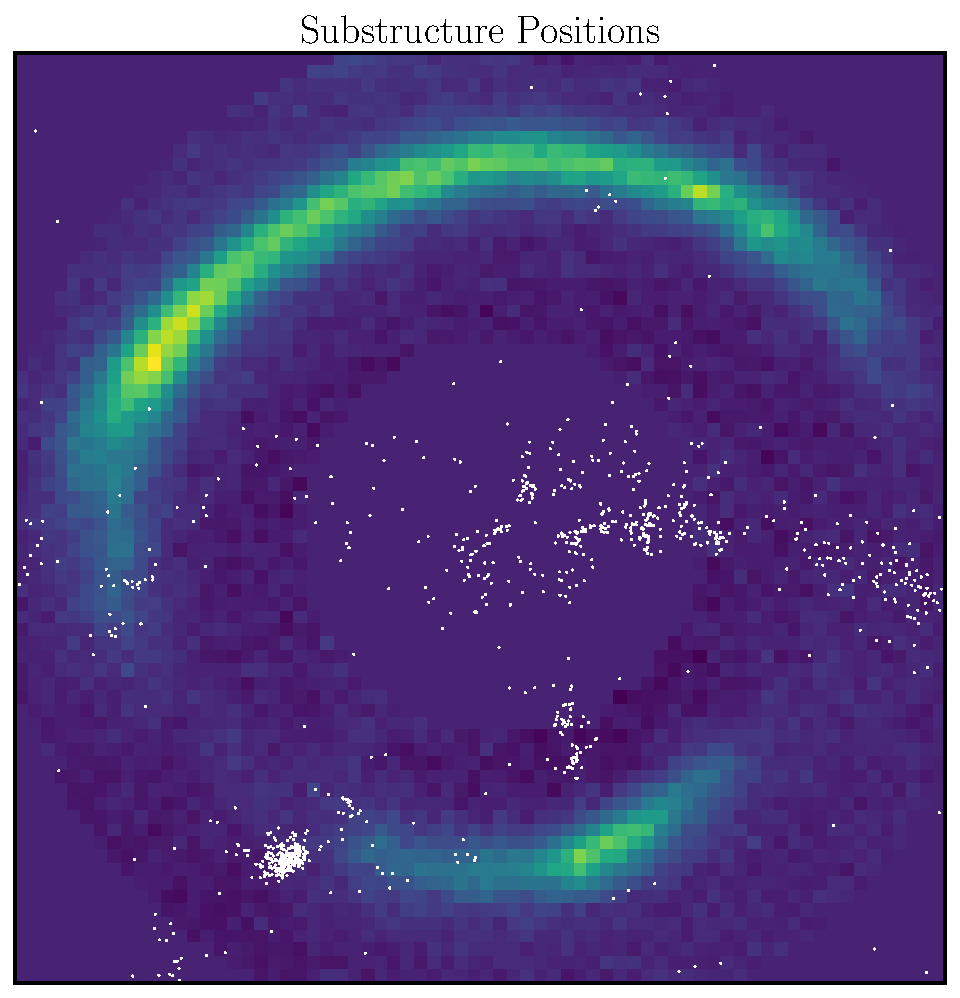
\includegraphics[scale=0.45]{substructures.pdf}
\caption{\label{fig:substructures}}
\end{figure}

\begin{figure}
\centering
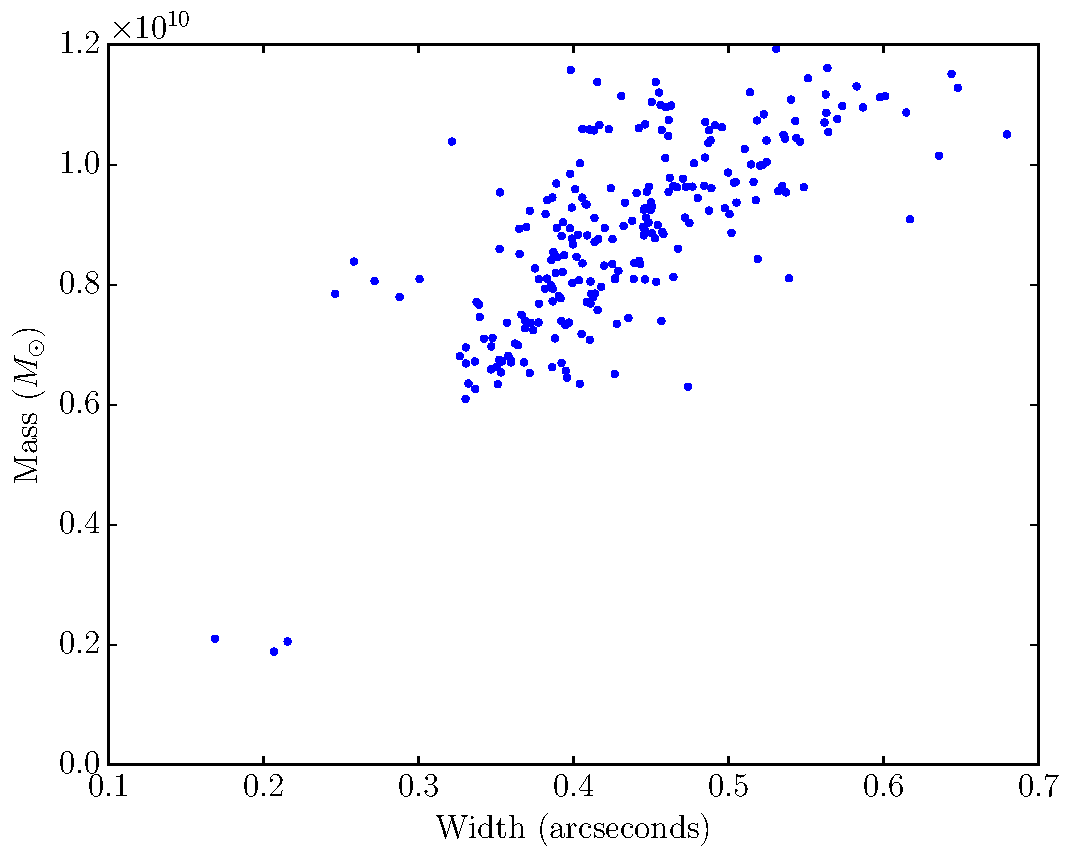
\includegraphics[scale=0.45]{mass_width.pdf}
\caption{\label{fig:mass_width}}
\end{figure}



\section*{Acknowledgements}
It is a pleasure to thank Matt Auger (Cambridge) for valuable discussion and
providing the data. Barkana

This work was funded by a Marsden Fast Start grant from the Royal Society of
New Zealand.


\begin{thebibliography}{99}
\end{thebibliography}


\end{document}

